\documentclass{article}
\usepackage[utf8]{inputenc}

\title{Laboratorio03_INTELIGENCIA_NEGOCIOS}
\author{edwartbalcon}
\date{Septiembre 2021}

\usepackage[utf8]{inputenc}
\usepackage[spanish]{babel}
\usepackage{natbib}
\usepackage{graphicx}

\begin{document}

\title{Caratula}

\begin{titlepage}
\begin{center}
\begin{Large}
\textbf{UNIVERSIDAD PRIVADA DE TACNA} \\
\end{Large}
\vspace*{-0.025in}
\begin{figure}[htb]
\begin{center}

\includegraphics[width=6cm]{./images/logo_UPT}
\end{center}
\end{figure}
\vspace*{-0.025in}
\begin{Large}
\textbf{FACULTAD DE INGENIERIA} \\
\end{Large}
\vspace*{0.05in}
\begin{Large}
\textbf{Escuela Profesional de Ingeniería de Sistema} \\
\end{Large}


\vspace*{0.4in}

\vspace*{0.1in}
\begin{Large}
\textbf{Informe de laboratorio 06: Kinesis Data Firehose} \\
\end{Large}

\vspace*{0.3in}
\begin{Large}
\textbf{Curso: Inteligencia de negocios} \\
\end{Large}

\vspace*{0.3in}
\begin{Large}
\textbf{DOCENTE: Ing. Patrick Cuadros Quiroga} \\
\end{Large}

\vspace*{0.2in}
\vspace*{0.1in}
\begin{large}

\begin{Large}
\textbf{Alumno: Balcon Coahila, Edwart Juan\hfill	(2013046516) } \\
\end{Large}

\vspace*{0.15in}
\begin{Large}
\textbf{Tacna – Perú} \\
\end{Large}

\vspace*{0.05in}
\begin{Large}
\textbf{2021 } \\
\end{Large}

\end{large}
\end{center}

\end{titlepage}


\newpage

\section{ Realizar los siguientes pasos para el laboratorio }

\textbf{1.1. Ingestando datos a Firehose mediante el SDK de AWS}

    \begin{center}
		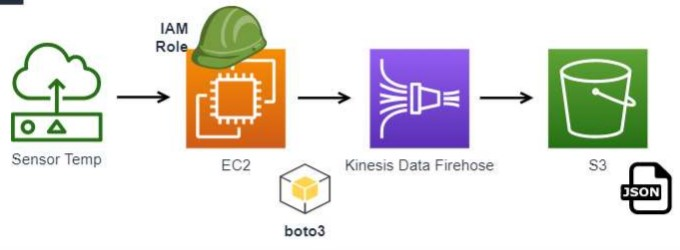
\includegraphics[width=15cm]{./images/1} 
	\end{center}
	
\textbf{1.2.  Entrar a la consola de AWS}

\textbf{1.3.  Ir al servicio de Kinesis Firehose, clic en Create delivery stream
}

    \begin{center}
		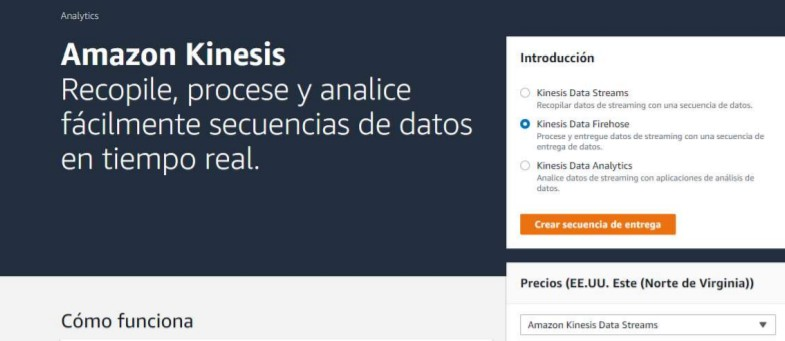
\includegraphics[width=15cm]{./images/2} 
	\end{center}

\newpage
\textbf{1.4.  Crear el stream con el nombre de StreamSensorIoT, y luego siguiente y otra vez siguiente.
}

    \begin{center}
		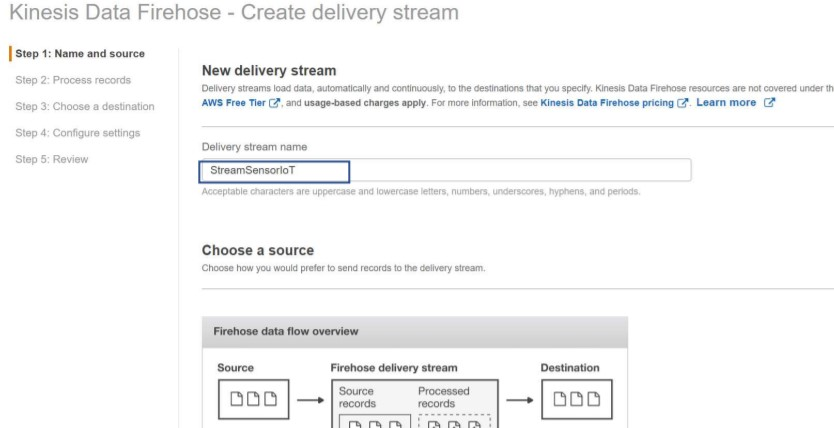
\includegraphics[width=15cm]{./images/3} 
	\end{center}
	
	\newpage
\textbf{1.5.   En la siguiente ventana, dejamos marcado S3, porque es ahí donde almacenaremos los datos que se
agregarán a Kinesis Data Firehose.
}

    \begin{center}
		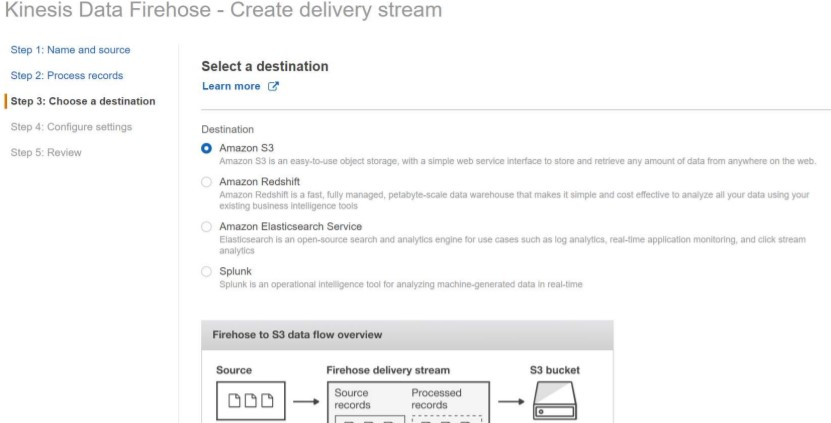
\includegraphics[width=15cm]{./images/4} 
	\end{center}
	
	\newpage
\textbf{1.6.  Creamos un bucket en la siguiente pantalla. (Los nombres de los bucket son únicos globalmente)
}

    \begin{center}
		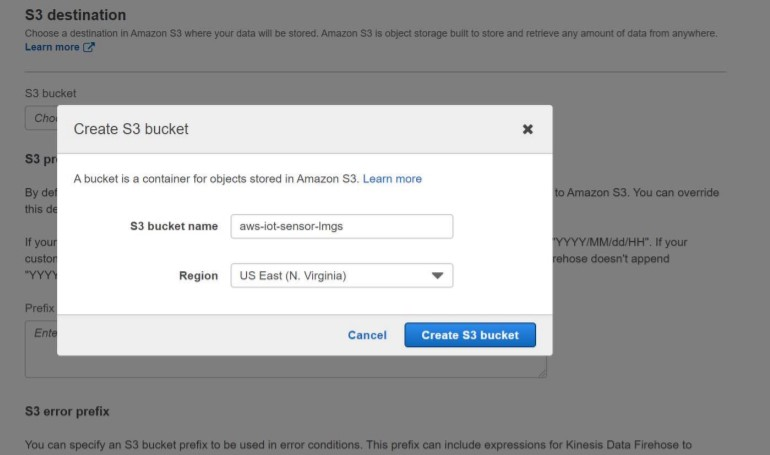
\includegraphics[width=15cm]{./images/5} 
	\end{center}
	 \begin{center}
		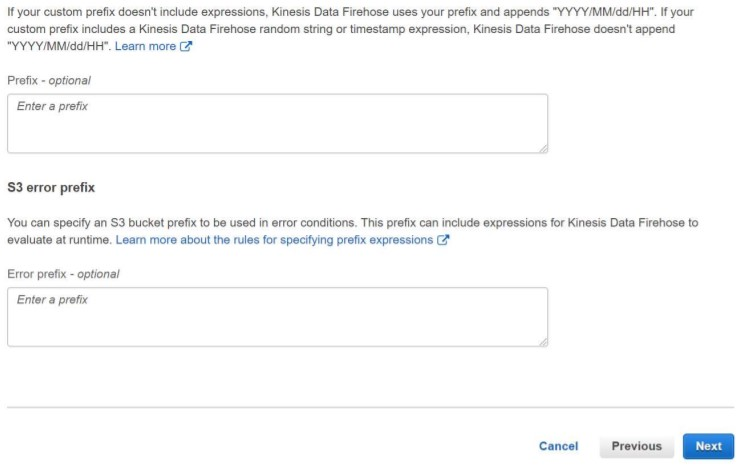
\includegraphics[width=15cm]{./images/6} 
	\end{center}
	
	\newpage
\textbf{1.7.  En la siguiente ventana, definimos que el tamaño del búfer será de 1MB y el intervalo de tiempo es de 60
segundos. (Recordar que al cumplirse una de estas dos condiciones los datos se guardarán en S3)
}

    \begin{center}
		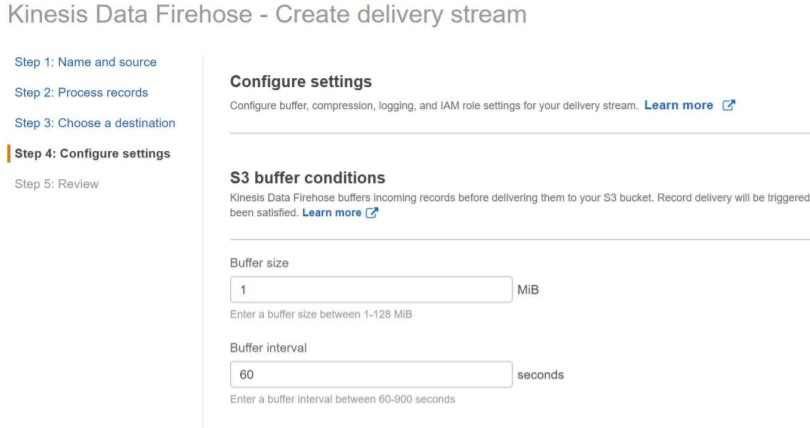
\includegraphics[width=15cm]{./images/7} 
	\end{center}
	
	\newpage
\textbf{1.8.  Seleccionamos la opción de crear un rol de IAM y Next. (Este rol, permitirá escribir los resultados en S3)
}

    \begin{center}
		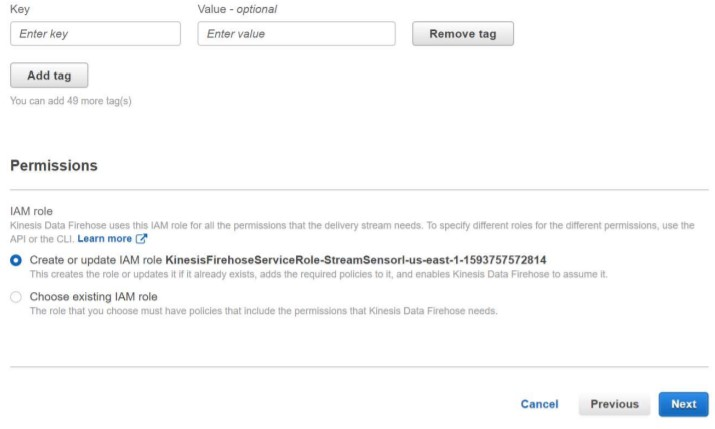
\includegraphics[width=15cm]{./images/8} 
	\end{center}
	
	\newpage
\textbf{1.9.  Siguiente y Crear delivery stream.
}

    \begin{center}
		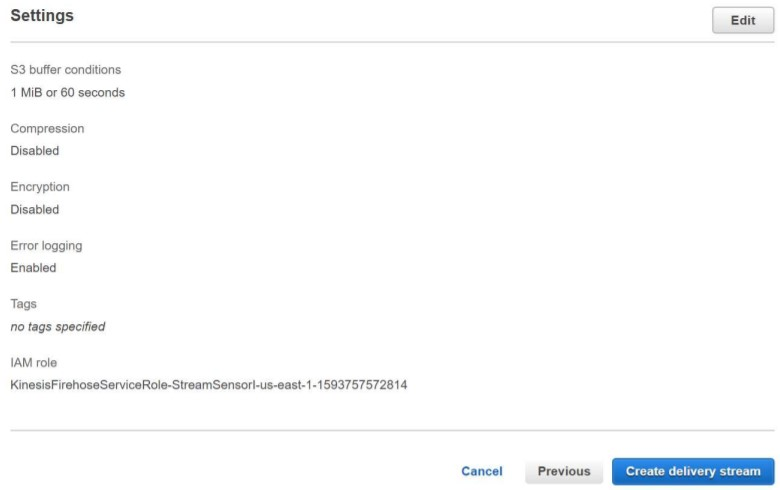
\includegraphics[width=15cm]{./images/9} 
	\end{center}
	
		
	\newpage
\textbf{1.10.  El stream en Kinesis Data Firehose se ha creado
}

    \begin{center}
		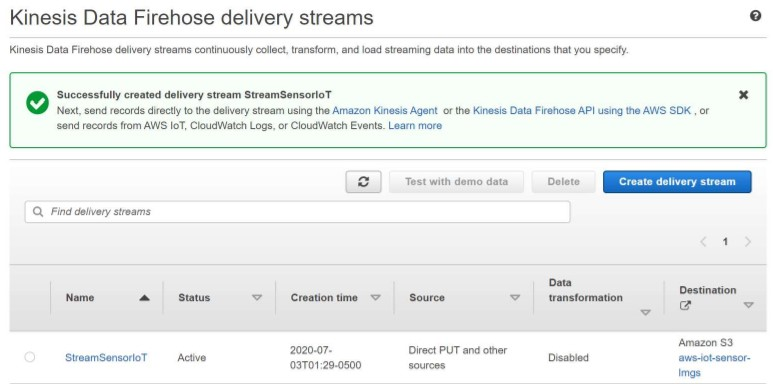
\includegraphics[width=15cm]{./images/10} 
	\end{center}
	
	
		
	\newpage
\textbf{1.11.  Entramos a Cloud9, clic en Open IDE.
}

    \begin{center}
		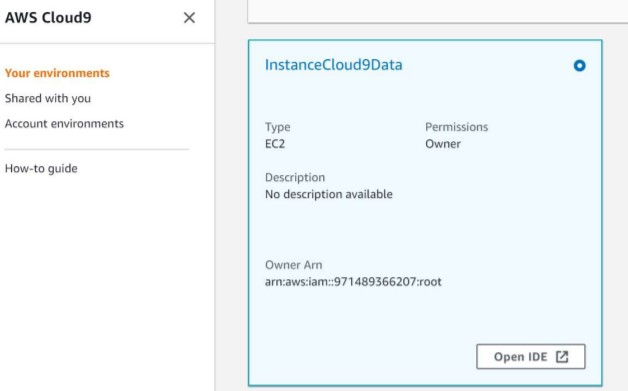
\includegraphics[width=15cm]{./images/11} 
	\end{center}
	
	

\end{document}